\chapter{\sc Two-Phase Stokes Flow Numerical Results}\label{ch:stokes_results}
In order to test our method, and to allow comparisons with the unfitted finite
element approximation in \cite{spurious}, we now present several numerical
experiments in 2d and 3d.

The chapter is organised as follows: in \S\ref{sec:stokes_exact_solutions} we
state two exact solutions to the two-phase Stokes problem and we verify that
they are indeed solutions; in \S\ref{sec:errors} we describe the general
settings for the simulations and we define the error estimators used; in
\S\ref{sec:stokes_2d_convergence_results} we report on the convergence test in
2d; in \S\ref{sec:stokes_2d_equidistributon} we show that interface mesh points
are naturally equidistributed by our scheme; in \S\ref{sec:stokes_2d_energy} we
show that our scheme conserve the enclosed volume and that the surface energy
monotonically decays; in \S\ref{sec:stokes_2d_shear} we present a shear
flow experiment in 2d; in \S\ref{sec:stokes_3d_convergence_results} we report on
the convergence test in 3d; in \S\ref{sec:stokes_3d_shear} we finally present a
shear flow experiment in 3d.

\section{Exact solutions}\label{sec:stokes_exact_solutions}
We recall the following stationary and expanding spherical solutions
from \cite{spurious}. Let $\Gamma(t) = \{ \vec z \in \R^d : |\vec z| = r(t)\}$
be a sphere of radius $r(t)$  and mean curvature $\varkappa(t) =
-\frac{d-1}{r(t)}$. Moreover let $\alpha,\gamma\in \R_{\geq 0}$ be given. We
will refer to (\ref{eq:radialr},b) as the stationary bubble solution, and to
(\ref{eq:radialr2},b) as the expanding bubble solution.

\subsection{Stationary bubble}
The stationary sphere where
\begin{subequations}
\begin{equation} \label{eq:radialr}
r(t) = r(0)\,,
\end{equation}
together with
\begin{equation} \label{eq:radialup}
\vec u(\vec z, t) = \vec 0 \,,\quad p(\vec z, t) =
-\,\gamma \varkappa(0)\left[\charfcn{\Omega_-(0)}
-\frac{\vol(\Omega_-(0))}{\vol(\Omega)} \right] ,
\end{equation}
\end{subequations}
is an exact solution to the problem (\ref{eq:stokes_full_momentum}--h) on e.g.\
$\Omega = (-1,1)^d$ with $\vec f=\vec 0$ and $\vec g = \vec 0$ on
$\partial_1\Omega=\partial\Omega$. This solution is the continuous version of
(\ref{eq:solsol}).

It is trivial to verify that (\ref{eq:radialr},b) is indeed an exact solution.
Firstly, given that the velocity $\vec u$ is constant and the pressure $p$ is
constant in each phase, the momentum equation (\ref{eq:stokes_full_momentum})
automatically holds if $\vec f=\vec 0$ and the mass equation
(\ref{eq:stokes_full_mass}) is satisfied. Finally, also the stress balance
(\ref{eq:stokes_full_jump_stress}) holds since, substituting
(\ref{eq:radialup}) in (\ref{eq:stokes_full_jump_stress}), we obtain
\begin{align*}
[2\mu \,\mat D(\vec u)\,.\,\vec\nu - p\,\vec \nu]_-^+ = & [- p\,\vec \nu]_-^+ \\
= & -\gamma \varkappa(0)\frac{\vol(\Omega_-(0))}{\vol(\Omega)}\vec \nu
-\gamma \varkappa(0)\vec \nu +
\gamma \varkappa(0)\frac{\vol(\Omega_-(0))}{\vol(\Omega)}\vec \nu \\
= & -\gamma \varkappa(0)\vec \nu\,.
\end{align*}
\subsection{Expanding bubble}
A nontrivial divergence free and radially symmetric solution $\vec u$ can be
constructed on a domain that does not contain the origin. To this end, consider
e.g. $\Omega = (-1,1)^d \setminus [-\frac13,\frac13]^d$. Then, the expanding
sphere where
\begin{subequations}
\begin{equation} \label{eq:radialr2}
r(t) = ([r(0)]^d + \alpha\,t\,d)^\frac1d \,,
\end{equation}
together with
\begin{equation} \label{eq:radialup2}
\vec u(\vec z, t) = \alpha\,\frac{\vec z}{|\vec z\,|^d}\,, \quad
p(\vec z, t) = -\,\bigg(\gamma +2\,\alpha\,\frac{\mu_+ - \mu_-}
{r(t)^{d-1}}\bigg)\,\varkappa(t)\,\left[ \charfcn{\Omega_-(t)} -
\frac{\vol(\Omega_-(t))}{\vol(\Omega)}\right],
\end{equation}
\end{subequations}
is an exact solution to the problem (\ref{eq:stokes_full_momentum}--h) with
$\vec f = \vec 0$ and $\vec g(\vec z) = \alpha\,|\vec z|^{-d}\,\vec z$ on
$\partial_1\Omega=\partial\Omega$.

We now verify that (\ref{eq:radialr2},b) is indeed an exact solution. Firstly,
we have that
\begin{equation*}
\frac{\partial u_i}{\partial z_j}=\alpha\frac{\delta_{ij}|\vec z\,|^d
- d z_i z_j |\vec z\,|^{d-2}}{|\vec z\,|^{2d}}\,.
\end{equation*}
Since $\frac{\partial u_i}{\partial z_j}=\frac{\partial u_j}{\partial z_i}$,
the components of the rate-of-deformation tensor are simply
\begin{equation*}
\big[\mat D(\vec u) \big]_{ij} = \frac{1}{2}\bigg(\frac{\partial
u_i}{\partial z_j} + \frac{\partial u_j}{\partial z_i}\bigg)=\frac{\partial
u_i}{\partial z_j}\,.
\end{equation*}
Then, it holds
\begin{align*}
\nabla\,.\,\mat D(\vec u) = & \sum_{i=1}^d\frac{\partial}{\partial z_i}
\frac{\partial u_i}{\partial z_i} = \alpha\sum_{i=1}^d \frac{\partial}{\partial
z_i}\big(|\vec z\,|^{-d}-dz_i^2|\vec z\,|^{-d-2}\big) \\
= & \alpha\sum_{i=1}^d\bigg[ -3dz_i|\vec z\,|^{-d-2}+dz_i^3(d+2)|
\vec z\,|^{-d-4}\bigg] \\
= & \alpha d |\vec z\,|^{-d-4}\sum_{i=1}^d\bigg[-3 z_i|\vec z\,|^2 +
(d+2)z_i^3\bigg]
\end{align*}

The mass equation (\ref{eq:stokes_full_mass}) is also satisfied since we have
\begin{equation*}
\nabla\,.\,\vec u=\sum_{i=1}^d\frac{\partial u_i}{\partial z_i} = \alpha
\sum_{i=1}^d\frac{|\vec z\,|^d - d z^2_i|\vec z\,|^{d-2}}{|\vec z \,|^{2d}} =
\alpha \frac{d|\vec z\,|^d - d |\vec z\,|^2|\vec z\,|^{d-2}}{|\vec z\,|^{2d}} =
0\,.
\end{equation*}

\section{Settings and error estimators}\label{sec:errors}
In our numerical simulations, unless otherwise stated, we use the following
settings. We choose the initial surface $\Gamma(0) = \{ \vec z \in \R^d : |\vec
z| = \frac12 \}$, the domain $\Omega = (-1,1)^d$ and we employ uniform time
steps $\tau_m=\tau$, $m=0,\ldots, M-1$. Moreover, we set the GMRES tolerance to
tol $=10^{-12}$ and the restart value to 50. We use the Stokes matrix
(\ref{eq:stokes_direct_precond}) or, depending on the pressure space,
(\ref{eq:stokes_direct_precond_extended}) as a preconditioner factorizing it
with UMFPACK. We point out that the restart value corresponds to the size
of the Krylov subspace used by the GMRES method while the tolerance is the
value for the stopping criterion. More precisely, the GMRES iteration ends when
the ratio between the norm of the preconditioned actual residual and the norm
of the preconditioned initial residual is smaller than the required tolerance.

We define the errors
\begin{equation} \label{eq:errorXx}
\errorXx := \max_{m=1,\ldots, M} \|\Gamma^m - \Gamma(t_m)\|_{L^\infty}\,,
\end{equation}
where $\|\Gamma^m - \Gamma(t_m)\|_{L^\infty} :=
\max_{k=1,\ldots, K_\Gamma} {\rm dist}( \vec q^m_k, \Gamma(t_m))$,
\begin{equation} \label{eq:errorLUu}
\LerrorUu2 := \left[\tau\,\sum_{m=1}^M \|\vec U^m - I^m_2\,\vec u(\cdot,
t_m)\|_{L^2(\Omega)}^2 \right]^\frac12,
\end{equation}
\begin{equation} \label{eq:errorHUu}
\HerrorUu2 := \left[\tau\,\sum_{m=1}^M \|\vec U^m - I^m_2\,\vec u(\cdot,
t_m)\|_{H^1(\Omega)}^2 \right]^\frac12,
\end{equation}
and
\begin{equation} \label{eq:errorPp}
\LerrorPp := \left[\tau\,\sum_{m=1}^M \|P^m - p(\cdot,t_m)\|_{L^2(\Omega)}^2
\right]^\frac12.
\end{equation}
In (\ref{eq:errorPp}) we employ a quadrature rule of degree $k$, with $k=13$ in
2d and $k=10$ in 3d, to compute the $L^2$--norms over $\Omega$.

Finally, we also define the estimated error of convergence EOC as
\begin{equation} \label{eq:eoc}
\mbox{EOC}=\frac{\ln{\frac{\mbox{error}_1}{\mbox{error}_0}}}
{\ln{\frac{\mbox{h}_1}{\mbox{h}_0}}}\,,
\end{equation}
where $\mbox{error}_1$ is the error computed on a triangulation finer that the
one used to compute $\mbox{error}_0$ while $\mbox{h}_1$ and $\mbox{h}_0$ are the
respective characteristic lengths.

\section{Convergence tests in 2d}\label{sec:stokes_2d_convergence_results}
For the true solution (\ref{eq:radialr},b) we choose $\mu = \gamma = 1$.
Therefore, the solution reduces to $r(t) =
\frac{1}{2}$, $\vec u(\cdot, t) = \vec 0$ and $p(t) = 2\,\charfcn{\Omega_-(0)} -
\frac{\pi}{8}$ for all $t \geq 0$. We approximate this stationary solution on
nearly uniform meshes that feature $J_\Gamma = 2^i$, $i=4,\ldots,7$, uniform
interface elements and $J_\Omega^0 = 224$, $1076$, $4240$, $17194$ bulk
elements, respectively. We show the initial mesh for $J_\Gamma = 32$ in
Figure~\ref{fig:meshes_uniform}.
\begin{figure}[htbp]
\centering
\includegraphics[width=.45\textwidth]{figures/stokes/mesh_uniform.ps}
\caption[Stokes 2d stationary bubble initial mesh]
{Initial mesh for the 2d stationary bubble problem with $J_\Gamma = 32$
interface elements.}
\label{fig:meshes_uniform}
\end{figure}
In addition, we use a uniform time step size $\tau=10^{-2}$.
We compute the discrete solutions to this stationary problem over the time
interval $[0,1]$, and report on the errors for the P2--P0, P2--P1, P2--\pdg
and P2--(P1+P0) elements in Tables~\ref{tab:stokes_stationary_2d_p2p0},
\ref{tab:stokes_stationary_2d_p2p1}, \ref{tab:stokes_stationary_2d_p2p1dg} and
\ref{tab:stokes_stationary_2d_p2p1p0}, respectively.
\begin{table*}
\center
\begin{tabular}{rllllr}
\hline
$J_\Gamma$ & $\errorXx$ & $\LerrorUu2$ & $\LerrorPp$ & EOC & CPU[s] \\
\hline
 16 & 0 & 0 & 3.22254e-01 &    - &    9 \\
 32 & 0 & 0 & 1.41195e-01 & 0.90 &   54 \\
 64 & 0 & 0 & 4.06438e-02 & 1.80 &  292 \\
128 & 0 & 0 & 2.60448e-02 & 0.64 & 1443 \\
\hline
\end{tabular}
\caption[Stokes 2d stationary bubble errors P2--P0]
{($\mu=\gamma=1$) Stationary bubble problem on $(-1,1)^2$ over the time
interval $[0,1]$ for the P2--P0 element.}
\label{tab:stokes_stationary_2d_p2p0}
\end{table*}
\begin{table*}
\center
\begin{tabular}{rllllr}
\hline
$J_\Gamma$ & $\errorXx$ & $\LerrorUu2$ & $\LerrorPp$ & EOC & CPU[s] \\
\hline
 16 & 2.41133e-02 & 9.35478e-03 & 5.75614e-01 &    - &    5 \\
 32 & 1.21789e-02 & 3.44473e-03 & 3.99457e-01 & 0.40 &   36 \\
 64 & 6.17055e-03 & 1.24629e-03 & 2.77632e-01 & 0.52 &  170 \\
128 & 2.97451e-03 & 4.41980e-04 & 1.96901e-01 & 0.50 & 1343 \\
\hline
\end{tabular}
\caption[Stokes 2d stationary bubble errors P2--P1]
{($\mu=\gamma=1$) Stationary bubble problem on $(-1,1)^2$ over the time
interval $[0,1]$ for the P2--P1 element.}
\label{tab:stokes_stationary_2d_p2p1}
\end{table*}
\begin{table*}
\center
\begin{tabular}{rllllr}
\hline
$J_\Gamma$ & $\errorXx$ & $\LerrorUu2$ & $\LerrorPp$ & EOC & CPU[s] \\
\hline
 16 & 0 & 0 & 3.22254e-01 &    - &    8 \\
 32 & 0 & 0 & 1.41195e-01 & 0.90 &   42 \\
 64 & 0 & 0 & 4.06438e-02 & 1.80 &  181 \\
128 & 0 & 0 & 2.60448e-02 & 0.64 & 1006 \\
\hline
\end{tabular}
\caption[Stokes 2d stationary bubble errors P2--\pdg]
{($\mu=\gamma=1$) Stationary bubble problem on $(-1,1)^2$ over the time
interval $[0,1]$ for the P2--\pdg element.}
\label{tab:stokes_stationary_2d_p2p1dg}
\end{table*}
\begin{table*}
 \center
\begin{tabular}{rllllr}
\hline
$J_\Gamma$ & $\errorXx$ & $\LerrorUu2$ & $\LerrorPp$ & EOC & CPU[s] \\
\hline
 16 & 0 & 0 & 3.22254e-01 &    - &   13 \\
 32 & 0 & 0 & 1.41195e-01 & 0.90 &   44 \\
 64 & 0 & 0 & 4.06438e-02 & 1.80 &  203 \\
128 & 0 & 0 & 2.60448e-02 & 0.64 & 2151 \\
\hline
\end{tabular}
\caption[Stokes 2d stationary bubble errors P2--(P1+P0)]
{($\mu=\gamma=1$) Stationary bubble problem on $(-1,1)^2$ over the time
interval $[0,1]$ for the P2--(P1+P0) element.}
\label{tab:stokes_stationary_2d_p2p1p0}
\end{table*}

We can clearly see that the stationary nature of the true solution
(\ref{eq:radialr},b) is captured exactly by our numerical method with the
P2--P0, the P2--\pdg and the P2--(P1+P0) element, see also
Figure~\ref{fig:2d_stationary_bubble} for a visualization of the discrete
pressure in the case $J_\Gamma = 32$. This is not surprising given the
result of Theorem~\ref{thm:stat2}, and the fact that we use an equidistributed
approximation $\Gamma^0$, which means that (\ref{eq:constcurv}) is satisfied.
Instead the element P2--P1 does not satisfy the hypothesis that
$\charfcn{\Omega^m_-}\in\pspace^m$ of Theorem~\ref{thm:stat2} and therefore the
true solution is not captured exactly. Moreover, since
$\charfcn{\Omega_-^h(t)}\not\in \mbox{ P1}$, the volume conservation property
of the semidiscrete scheme (\ref{eq:stokes_volume_semidiscrete}) does not hold
which implies that the P2--P1 element does not conserve the enclosed volume. Of
course, since the discrete solution is stationary, neither smoothing nor
remeshing is performed for the simulations in
Tables~\ref{tab:stokes_stationary_2d_p2p0},
\ref{tab:stokes_stationary_2d_p2p1}, \ref{tab:stokes_stationary_2d_p2p1dg} and
\ref{tab:stokes_stationary_2d_p2p1p0}. We also observe that the error for the
three approximations with the P2--P0, the P2--\pdg and the P2--(P1+P0)
element, respectively, produce identical errors. Again, that is to be expected,
since the pressure solution (\ref{eq:solsol})
\begin{equation*}
P^{m+1} = -\gamma\,\overline\kappa\left[\charfcn{\Omega_-^m}
- \frac{\vol(\Omega_-^m)}{\vol(\Omega)}\right]
\end{equation*}
is such that $P^{m+1}$ is independent of $\pspace^m$, and so the additional
degrees of freedom are not utilized by the pressure approximation.
\begin{figure}[htbp]
\centering
\includegraphics[width=.45\textwidth]
{figures/stokes/2d_stationary_bubble_uniform_100.ps}
\caption[Stokes 2d stationary bubble pressure]
{($\mu=\gamma=1$) Pressure of the 2d stationary bubble at time $t=1$
for the P2--P0 element.}
\label{fig:2d_stationary_bubble}
\end{figure}

For the expanding bubble test, we fix $\Omega = (-1,1)^2 \setminus
[-\frac13,\frac13]^2$ and we choose the parameters $\alpha = 0.15$ and $\mu_+ =
10\,\mu_- = \gamma = 1$ for the true solution (\ref{eq:radialr2},b). Here we
consider two different bulk mesh strategies. Either we use a nearly uniform
mesh, as shown on the left of Figure~\ref{fig:meshes_expanding}, or an adaptive
mesh that uses a finer resolution close to the interface, see the example mesh
on the right-hand side of Figure~\ref{fig:meshes_expanding}.
\begin{figure}[htbp]
\centering
\subfloat[Uniform mesh with $J_\Gamma = 32$]{
\includegraphics[width=.45\textwidth]{figures/stokes/mesh_hole_uniform.ps}}
\subfloat[Adaptive mesh with $J_\Gamma = 64$]{
\includegraphics[width=.45\textwidth]{figures/stokes/mesh_hole_adaptive.ps}}
\caption[Stokes 2d expanding bubble initial meshes]
{Initial meshes for the expanding bubble problem.}
\label{fig:meshes_expanding}
\end{figure}

Details on the discretization parameters for the nearly uniform meshes are
given in Table~\ref{tab:expandingbubble2Delements}. Here we explicitly
state the final number of bulk elements, $J_\Omega^M$, in the case $C_v = 1$
and $C_v = 3$, recall the remesh criterion (\ref{eq:volume_criterion}). In the
former the bulk is remeshed after every time step while in the latter the bulk
is remeshed when the max--min entity volume ratio is bigger than 3. Of course,
when only smoothing is employed, then the number of bulk mesh elements is
invariant, and so $J_\Omega^M = J_\Omega^0$.
\begin{table*}
\center
\begin{tabular}{rrrrr}
\hline
$J_\Gamma$ & $J_\Omega^0$ & $\tau$ & $J_\Omega^M$ for $C_v=1$ &
$J_\Omega^M$ for $C_v=3$ \\
\hline
 16 &   316 & $1.6\cdot10^{-2}$ &  120 &  184 \\
 32 &  1016 &   $4\cdot10^{-3}$ &  452 &  468 \\
 64 &  3916 &         $10^{-3}$ & 1864 & 1858 \\
128 & 15784 & $2.5\cdot10^{-4}$ & 7264 & 7263 \\
\hline
\end{tabular}
\caption[Stokes expanding bubble uniform meshes parameters]
{Discretization parameters for the 2d expanding bubble problem, nearly uniform
meshes.}
\label{tab:expandingbubble2Delements}
\end{table*}
We report on the error for the P2--P0, the P2--\pdg and the P2--(P1+P0)
element in Table~\ref{tab:expandingbubble2Dp2p0},
\ref{tab:expandingbubble2Dp2p1dg} and \ref{tab:expandingbubble2Dp2p1p0},
respectively. On the top part of the tables only mesh smoothings are applied,
in the central part the bulk mesh is remeshed after every time step while at
the bottom the bulk mesh is remeshed only when the criterion
(\ref{eq:volume_criterion}), with $C_v=3$, is not satisfied.
\begin{table*}
\center
\hspace*{-3.25cm}
\begin{tabular}{rllllllr}
\hline
$J_\Gamma$ & $\errorXx$ & $\LerrorUu2$ & EOC & $\HerrorUu2$ & $\LerrorPp$ & EOC
& CPU[s] \\
\hline
& \multicolumn{7}{c}{no remeshing} \\
\hline
 16 & 5.94637e-03 & 7.26038e-04 &    - & 1.98118e-02 & 4.30560e-01 &    - &
9 \\
 32 & 1.47959e-03 & 3.39540e-04 & 0.83 & 1.17665e-02 & 2.27294e-01 & 0.70 &
98 \\
 64 & 3.68960e-04 & 8.66188e-05 & 1.97 & 5.82989e-03 & 1.05041e-01 & 1.11 &
1709 \\
128 & 9.20414e-05 & 5.87165e-05 & 0.56 & 6.24063e-03 & 3.18072e-02 & 1.72 &
37539 \\
\hline
& \multicolumn{7}{c}{$C_v=1$} \\
\hline
 16 & 5.92441e-03 & 5.27627e-04 &    - & 1.57505e-02 & 4.43442e-01 &    - &
59 \\
 32 & 1.46657e-03 & 1.05800e-04 & 1.75 & 5.26275e-03 & 2.14680e-01 & 0.79 &
100 \\
 64 & 3.65433e-04 & 1.48680e-05 & 2.83 & 1.50695e-03 & 8.14177e-02 & 1.40 &
2785 \\
128 & 9.12526e-05 & 1.81107e-06 & 3.04 & 3.59374e-04 & 3.69593e-02 & 1.14 &
23465 \\
\hline
& \multicolumn{7}{c}{$C_v=3$} \\
\hline
 16 & 5.94589e-03 & 5.71201e-04 &    - & 1.51195e-02 & 4.44395e-01 &    - &
41 \\
 32 & 1.47176e-03 & 1.02091e-04 & 1.88 & 4.86975e-03 & 2.13617e-01 & 0.80 &
92 \\
 64 & 3.65488e-04 & 1.50366e-05 & 2.76 & 1.50058e-03 & 8.22797e-02 & 1.38 &
1847 \\
128 & 9.12406e-05 & 1.81327e-06 & 3.05 & 3.59347e-04 & 3.69473e-02 & 1.16 &
26973 \\
\hline
\end{tabular}
\hspace*{-3.25cm}
\caption[Stokes expanding bubble uniform mesh errors P2--P0]
{($\mu_+ = 10\,\mu_- = \gamma = 1,\alpha = 0.15$) Expanding bubble
problem on $(-1,1)^2\setminus[-\frac{1}{3},\frac{1}{3}]^2$ over the time
interval $[0,1]$ for the P2--P0 element with nearly uniform mesh.}
\label{tab:expandingbubble2Dp2p0}
\end{table*}
\begin{table*}
\center
\hspace*{-3.25cm}
\begin{tabular}{rllllllr}
\hline
$J_\Gamma$ & $\errorXx$ & $\LerrorUu2$ & EOC & $\HerrorUu2$ & $\LerrorPp$ & EOC
& CPU[s] \\
\hline
& \multicolumn{7}{c}{no remeshing} \\
\hline
 16 & 5.99881e-03 & 1.42557e-03 &    - & 3.45859e-02 & 4.31784e-01 &    - &
9 \\
 32 & 1.47936e-03 & 4.11514e-04 & 1.36 & 1.28088e-02 & 2.27350e-01 & 0.70 &
82 \\
 64 & 3.69030e-04 & 1.03424e-04 & 1.99 & 6.17291e-03 & 1.05060e-01 & 1.11 &
1391 \\
128 & 9.21619e-05 & 6.12532e-05 & 0.76 & 6.21616e-03 & 3.17967e-02 & 1.72 &
31042 \\
\hline
& \multicolumn{7}{c}{$C_v=1$} \\
\hline
 16 & 5.95848e-03 & 8.38757e-04 &    - & 2.23968e-02 & 4.44061e-01 &    - &
100 \\
 32 & 1.47123e-03 & 2.22736e-04 & 1.45 & 7.70628e-03 & 2.15081e-01 & 0.79 &
728 \\
 64 & 3.65750e-04 & 2.16681e-05 & 3.36 & 1.76987e-03 & 8.15608e-02 & 1.40 &
3050 \\
128 & 9.12893e-05 & 2.33116e-06 & 3.22 & 3.96930e-04 & 3.69418e-02 & 1.14 &
25348 \\
\hline
& \multicolumn{7}{c}{$C_v=3$} \\
\hline
 16 & 5.99703e-03 & 8.59166e-04 &    - & 2.23227e-02 & 4.44656e-01 &    - &
47 \\
 32 & 1.47622e-03 & 2.03051e-04 & 1.57 & 7.04524e-03 & 2.13800e-01 & 0.80 &
145 \\
 64 & 3.65886e-04 & 2.21067e-05 & 3.20 & 1.77973e-03 & 8.20109e-02 & 1.38 &
2325 \\
128 & 9.12664e-05 & 2.33913e-06 & 3.24 & 3.97020e-04 & 3.69351e-02 & 1.15 &
26045 \\
\hline
\end{tabular}
\hspace*{-3.25cm}
\caption[Stokes expanding bubble uniform mesh errors P2--\pdg]
{($\mu_+ = 10\,\mu_- = \gamma = 1,\alpha = 0.15$) Expanding bubble
problem on $(-1,1)^2\setminus[-\frac{1}{3},\frac{1}{3}]^2$ over the time
interval $[0,1]$ for the P2--\pdg element with nearly uniform mesh.}
\label{tab:expandingbubble2Dp2p1dg}
\end{table*}
\begin{table*}
\center
\hspace*{-3.25cm}
\begin{tabular}{rllllllr}
\hline
$J_\Gamma$ & $\errorXx$ & $\LerrorUu2$ & EOC & $\HerrorUu2$ & $\LerrorPp$ & EOC
& CPU[s] \\
\hline
& \multicolumn{7}{c}{no remeshing} \\
\hline
 16 & 5.99532e-03 & 1.55402e-03 &    - & 4.09186e-02 & 4.31782e-01 &    - &
9 \\
 32 & 1.48145e-03 & 4.40335e-04 & 1.38 & 1.35501e-02 & 2.27375e-01 & 0.70 &
80 \\
 64 & 3.68601e-04 & 1.08675e-04 & 2.02 & 6.48883e-03 & 1.05064e-01 & 1.11 &
1316 \\
128 & 9.22254e-05 & 6.25696e-05 & 0.80 & 6.07813e-03 & 3.17870e-02 & 1.72 &
39375 \\
\hline
& \multicolumn{7}{c}{$C_v=1$} \\
\hline
 16 & 5.96235e-03 & 8.94203e-04 &    - & 2.61842e-02 & 4.44306e-01 &    - &
159 \\
 32 & 1.47265e-03 & 2.41779e-04 & 1.43 & 1.03858e-02 & 2.15011e-01 & 0.79 &
619 \\
 64 & 3.65605e-04 & 2.33308e-05 & 3.37 & 2.02208e-03 & 8.11222e-02 & 1.41 &
3014 \\
128 & 9.12693e-05 & 2.42966e-06 & 3.26 & 4.31820e-04 & 3.69632e-02 & 1.13 &
22128 \\
\hline
& \multicolumn{7}{c}{$C_v=3$} \\
\hline
 16 & 5.97343e-03 & 8.91171e-04 &    - & 2.46402e-02 & 4.45063e-01 &    - &
95 \\
 32 & 1.47254e-03 & 2.20844e-04 & 1.52 & 9.55901e-03 & 2.13809e-01 & 0.80 &
178 \\
 64 & 3.65587e-04 & 2.33348e-05 & 3.24 & 2.00192e-03 & 8.17655e-02 & 1.39 &
2225 \\
128 & 9.12663e-05 & 2.44147e-06 & 3.26 & 4.32699e-04 & 3.69512e-02 & 1.15 &
23265 \\
\hline
\end{tabular}
\hspace*{-3.25cm}
\caption[Stokes expanding bubble uniform mesh errors P2--(P1+P0)]
{($\mu_+ = 10\,\mu_- = \gamma = 1,\alpha = 0.15$) Expanding bubble
problem on $(-1,1)^2\setminus[-\frac{1}{3},\frac{1}{3}]^2$ over the time
interval $[0,1]$ for the P2--(P1+P0) element with nearly uniform mesh.}
\label{tab:expandingbubble2Dp2p1p0}
\end{table*}
Due to the expanding motion of the interface, if no remesh is used, we observe
that over time bulk mesh elements strongly deform. This leads to large CPU
times and additional approximation errors. In particular, the strong mesh
deformations for the finest run, with $J_\Omega^0 = J_\Omega^M = 15212$, leads
to a breakdown of the convergence rate for the $L^2$-velocity error, and, for
the elements P2--P0 and P2--\pdg, an actual increase in the $H^1$-velocity
error. Instead, if remesh is applied, we observe a dramatic improvement in the
CPU times, and a significant reduction in the error quantities. In particular,
there is no deterioration of the observed convergence rates. Comparing the
errors in Tables~\ref{tab:expandingbubble2Dp2p0},
\ref{tab:expandingbubble2Dp2p1dg} and \ref{tab:expandingbubble2Dp2p1p0} we note
that element P2--\pdg and element P2--(P1+P0) performs, in term of CPU times
and errors, almost the same and they are slightly outperformed by element
P2--P0, which, together with a a remesh performed at every time step, gives the
best overall results.

The evolution of the discrete pressure solution in the case $J_\Gamma = 32$,
for the run with $C_v = 1$, can be seen in
Figure~\ref{fig:expanding_bubble_uniform}.
\begin{figure}[htbp]
\centering
\subfloat[$t=0$]{\includegraphics[width=.45\textwidth]
{figures/stokes/expanding_bubble_uniform_remesh_000.ps}}\\
\subfloat[$t=0.25$]{\includegraphics[width=.45\textwidth]
{figures/stokes/expanding_bubble_uniform_remesh_025.ps}}
\subfloat[$t=0.5$]{\includegraphics[width=.45\textwidth]
{figures/stokes/expanding_bubble_uniform_remesh_050.ps}}\\
\subfloat[$t=0.75$]{\includegraphics[width=.45\textwidth]
{figures/stokes/expanding_bubble_uniform_remesh_075.ps}}
\subfloat[$t=1$]{\includegraphics[width=.45\textwidth]
{figures/stokes/expanding_bubble_uniform_remesh_100.ps}}
\caption[Stokes expanding bubble pressure uniform mesh]
{($\mu_+ = 10\,\mu_- = \gamma = 1,\alpha = 0.15$) Pressure evolution of
the 2d expanding bubble for the P2--P0 element, nearly uniform mesh.}
\label{fig:expanding_bubble_uniform}
\end{figure}
Here we note that the discontinuous jump in the pressure at the interface is
captured very well, with no oscillations being present. This is a significant
improvement on the oscillations observed in the discrete pressures for the
unfitted finite element approximation from \cite{spurious}, see e.g.\
Figure~6 in that paper.

Finally, we would also like to investigate the effect of using adaptive bulk
meshes, that are refined close to the interface. An example mesh is shown on
the right-hand side of Figure~\ref{fig:meshes_expanding}, and we list our
employed discretization parameters in
Table~\ref{tab:expandingbubble2Delements_adaptive}. Obviously the remesh
criterion (\ref{eq:volume_criterion}) cannot be used for an adaptive mesh since
it would be always violated therefore we use the angle criterion
(\ref{eq:angle_criterion}) with $C_a=20$\textdegree.
\begin{table*}
\center
\begin{tabular}{rrrrr}
\hline
$J_\Gamma$ & $J_\Omega^0$ & $\tau$ & $J_\Omega^M$ for $C_a=60$\textdegree &
$J_\Omega^M$ for $C_a=20$\textdegree \\
\hline
 32 &  460 & $6.4\cdot10^{-2}$ &  216 &  216 \\
 64 & 1040 & $1.6\cdot10^{-2}$ &  452 &  440 \\
128 & 2628 &   $4\cdot10^{-3}$ & 1084 & 1384 \\
256 & 7460 &         $10^{-3}$ & 3840 & 4004 \\
\hline
\end{tabular}
\caption[Stokes expanding bubble adaptive meshes parameters]{Discretization
parameters for the 2d expanding bubble problem, adaptive meshes.}
\label{tab:expandingbubble2Delements_adaptive}
\end{table*}
The observed errors for our numerical approximation are shown in
Table~\ref{tab:expandingbubble2Dp2p0adaptive},
\ref{tab:expandingbubble2Dp2p1dgadaptive} and
\ref{tab:expandingbubble2Dp2p1p0adaptive}.
\begin{table*}
\center
\hspace*{-3.25cm}
\begin{tabular}{rllllllr}
\hline
$J_\Gamma$ & $\errorXx$ & $\LerrorUu2$ & EOC & $\HerrorUu2$ & $\LerrorPp$ & EOC
& CPU[s] \\
\hline
& \multicolumn{7}{c}{no remeshing} \\
\hline
 32 & 4.37607e-03 & 8.78021e-04 &    - & 1.81156e-02 & 5.74936e-01 &    - &
3 \\
 64 & 9.85447e-04 & 1.01294e-04 & 3.12 & 5.67749e-03 & 2.79462e-01 & 1.04 &
18 \\
128 & 2.42678e-04 & 2.92289e-05 & 1.79 & 2.75563e-03 & 1.48572e-01 & 0.91 &
221 \\
256 & 6.09781e-05 & 2.55111e-05 & 0.19 & 2.58915e-03 & 7.95637e-02 & 0.88 &
3652 \\
\hline
& \multicolumn{7}{c}{$C_a=60$\textdegree} \\
\hline
 32 & 3.91561e-03 & 7.10756e-04 &    - & 1.60401e-02 & 5.58280e-01 &    - &
18 \\
 64 & 1.00456e-03 & 3.71590e-04 & 0.94 & 1.11137e-02 & 2.94466e-01 & 0.92 &
113 \\
128 & 2.48565e-04 & 2.67810e-04 & 0.47 & 9.27231e-03 & 1.50823e-01 & 0.97 &
644 \\
256 & 6.04620e-05 & 7.00763e-05 & 1.89 & 3.87511e-03 & 6.32475e-02 & 1.23 &
3877 \\
\hline
& \multicolumn{7}{c}{$C_a=20$\textdegree} \\
\hline
 32 & 3.96937e-03 & 7.08593e-04 &    - & 1.55497e-02 & 5.62013e-01 &    - &
4 \\
 64 & 1.00880e-03 & 2.93799e-04 & 1.27 & 8.94937e-03 & 2.87566e-01 & 0.97 &
15 \\
128 & 2.43658e-04 & 1.44371e-04 & 1.03 & 5.72647e-03 & 1.53910e-01 & 0.90 &
154 \\
256 & 6.10778e-05 & 6.57476e-05 & 1.11 & 3.81816e-03 & 6.73295e-02 & 1.17 &
1441 \\
\hline
\end{tabular}
\hspace*{-3.25cm}
\caption[Stokes expanding bubble adaptive mesh errors P2--P0]
{($\mu_+ = 10\,\mu_- = \gamma = 1,\alpha = 0.15$) Expanding bubble
problem on $(-1,1)^2\setminus[-\frac{1}{3},\frac{1}{3}]^2$ over the time
interval $[0,1]$ for the P2--P0 element with adaptive mesh.}
\label{tab:expandingbubble2Dp2p0adaptive}
\end{table*}
\begin{table*}
\center
\hspace*{-3.25cm}
\begin{tabular}{rllllllr}
\hline
$J_\Gamma$ & $\errorXx$ & $\LerrorUu2$ & EOC & $\HerrorUu2$ & $\LerrorPp$ & EOC
& CPU[s] \\
\hline
& \multicolumn{7}{c}{no remeshing} \\
\hline
 32 & 4.44770e-03 & 1.03835e-03 &    - & 2.09015e-02 & 5.74058e-01 &    - &
2 \\
 64 & 9.96385e-04 & 1.24152e-04 & 3.06 & 5.85650e-03 & 2.79564e-01 & 1.04 &
22 \\
128 & 2.43860e-04 & 3.43865e-05 & 1.85 & 2.92915e-03 & 1.48563e-01 & 0.91 &
209 \\
256 & 6.09133e-05 & 2.85605e-05 & 0.26 & 2.71585e-03 & 7.95602e-02 & 0.88 &
4281 \\
\hline
& \multicolumn{7}{c}{$C_a=60$\textdegree} \\
\hline
 32 & 4.04836e-03 & 1.03041e-03 &    - & 2.11862e-02 & 5.58428e-01 &    - &
13 \\
 64 & 1.06336e-03 & 5.81260e-04 & 0.83 & 1.47843e-02 & 2.94451e-01 & 0.92 &
52 \\
128 & 2.64772e-04 & 4.48334e-04 & 0.37 & 1.27870e-02 & 1.50552e-01 & 0.97 &
364 \\
256 & 6.39800e-05 & 1.38724e-04 & 1.65 & 5.44161e-03 & 6.32714e-02 & 1.22 &
3743 \\
\hline
& \multicolumn{7}{c}{$C_a=20$\textdegree} \\
\hline
 32 & 4.08914e-03 & 9.75075e-04 &    - & 1.98793e-02 & 5.63360e-01 &    - &
5 \\
 64 & 1.05303e-03 & 4.43826e-04 & 1.14 & 1.14591e-02 & 2.87514e-01 & 0.97 &
13 \\
128 & 2.50894e-04 & 2.89007e-04 & 0.62 & 8.72470e-03 & 1.54031e-01 & 0.90 &
148 \\
256 & 6.40185e-05 & 1.15617e-04 & 1.29 & 5.10565e-03 & 6.98979e-02 & 1.11 &
2143 \\
\hline
\end{tabular}
\hspace*{-3.25cm}
\caption[Stokes expanding bubble adaptive mesh errors P2--\pdg]
{($\mu_+ = 10\,\mu_- = \gamma = 1,\alpha = 0.15$) Expanding bubble
problem on $(-1,1)^2\setminus[-\frac{1}{3},\frac{1}{3}]^2$ over the time
interval $[0,1]$ for the P2--\pdg element with adaptive mesh.}
\label{tab:expandingbubble2Dp2p1dgadaptive}
\end{table*}
\begin{table*}
\center
\hspace*{-3.25cm}
\begin{tabular}{rllllllr}
\hline
$J_\Gamma$ & $\errorXx$ & $\LerrorUu2$ & EOC & $\HerrorUu2$ & $\LerrorPp$ & EOC
& CPU[s] \\
\hline
& \multicolumn{7}{c}{no remeshing} \\
\hline
 32 & 4.39967e-03 & 1.14087e-03 &    - & 2.26396e-02 & 5.73270e-01 &    - &
6 \\
 64 & 9.94365e-04 & 1.34986e-04 & 3.08 & 6.01358e-03 & 2.79584e-01 & 1.04 &
25 \\
128 & 2.43769e-04 & 3.91547e-05 & 1.79 & 3.13728e-03 & 1.48565e-01 & 0.91 &
210 \\
256 & 6.08641e-05 & 3.20203e-05 & 0.28 & 2.77934e-03 & 7.95609e-02 & 0.88 &
3798 \\
\hline
& \multicolumn{7}{c}{$C_a=60$\textdegree} \\
\hline
 32 & 3.97673e-03 & 1.16740e-03 &    - & 2.54389e-02 & 5.59015e-01 &    - &
18 \\
 64 & 1.04465e-03 & 6.57166e-04 & 0.83 & 1.84165e-02 & 2.94657e-01 & 0.92 &
81 \\
128 & 2.64078e-04 & 5.07829e-04 & 0.37 & 1.60658e-02 & 1.50595e-01 & 0.97 &
385 \\
256 & 6.39339e-05 & 1.55008e-04 & 1.67 & 7.26636e-03 & 6.33057e-02 & 1.22 &
3274 \\
\hline
& \multicolumn{7}{c}{$C_a=20$\textdegree} \\
\hline
 32 & 4.02881e-03 & 1.12100e-03 &    - & 2.32002e-02 & 5.63527e-01 &    - &
4 \\
 64 & 1.04388e-03 & 5.00129e-04 & 1.16 & 1.39060e-02 & 2.85520e-01 & 0.98 &
18 \\
128 & 2.49831e-04 & 3.25755e-04 & 0.62 & 1.17532e-02 & 1.54026e-01 & 0.89 &
172 \\
256 & 6.45554e-05 & 1.34537e-04 & 1.25 & 6.48976e-03 & 6.98821e-02 & 1.11 &
2701 \\
\hline
\end{tabular}
\hspace*{-3.25cm}
\caption[Stokes expanding bubble adaptive mesh errors P2--(P1+P0)]
{($\mu_+ = 10\,\mu_- = \gamma = 1,\alpha = 0.15$) Expanding bubble
problem on $(-1,1)^2\setminus[-\frac{1}{3},\frac{1}{3}]^2$ over the time
interval $[0,1]$ for the P2--(P1+P0) element with adaptive mesh.}
\label{tab:expandingbubble2Dp2p1p0adaptive}
\end{table*}
Comparing the error quantities in Tables~\ref{tab:expandingbubble2Dp2p0},
\ref{tab:expandingbubble2Dp2p1dg} and \ref{tab:expandingbubble2Dp2p1p0}
against the ones in Tables~\ref{tab:expandingbubble2Dp2p0adaptive},
\ref{tab:expandingbubble2Dp2p1dgadaptive} and
\ref{tab:expandingbubble2Dp2p1p0adaptive} we note that there appears to
be no advantage in using a highly refined mesh near the moving interface. Again
the element which performs better in term of errors is the P2--P0 element
which, together with the choice of $C_a=20$\textdegree, gives the best result
in terms of accuracy and performance.

The evolution of the discrete pressure solution in the case $J_\Gamma = 64$, for
the run with $C_a=60$\textdegree, can be seen in
Figure~\ref{fig:expanding_bubble_adaptive}.
\begin{figure}[htbp]
\centering
\subfloat[$t=0$]{\includegraphics[width=.45\textwidth]
{figures/stokes/expanding_bubble_adaptive_remesh_000.ps}}\\
\subfloat[$t=0.25$]{\includegraphics[width=.45\textwidth]
{figures/stokes/expanding_bubble_adaptive_remesh_025.ps}}
\subfloat[$t=0.5$]{\includegraphics[width=.45\textwidth]
{figures/stokes/expanding_bubble_adaptive_remesh_050.ps}}\\
\subfloat[$t=0.75$]{\includegraphics[width=.45\textwidth]
{figures/stokes/expanding_bubble_adaptive_remesh_075.ps}}
\subfloat[$t=1$]{\includegraphics[width=.45\textwidth]
{figures/stokes/expanding_bubble_adaptive_remesh_100.ps}}
\caption[Stokes expanding bubble pressure adaptive mesh]
{($\mu_+ = 10\,\mu_- = \gamma = 1,\alpha = 0.15$) Pressure evolution of
the 2d expanding bubble for the P2--P0 element, adaptive mesh.}
\label{fig:expanding_bubble_adaptive}
\end{figure}

\section{Equidistribution property in 2d}\label{sec:stokes_2d_equidistributon}
We now demonstrate the remarkable equidistribution property of our method
showing that the circular, equidistributed numerical steady state solution is
recovered by our method even if we choose a very nonuniform initial interface
$\Gamma^0$. This is the analogue of what shown in \S\ref{subsec:sd_circle}
for a pure geometric PDE. In particular, for the presented numerical
simulation, we take $\Gamma^0$ to be a very nonuniform approximation of a unit
circle, where we represent the upper half of the circle by a single vertex,
while the lower half resembles a semicircle. In total we use $J_\Gamma = 32$
elements for $\Gamma^0$ and we start with a very nonuniform bulk mesh with
$J_\Omega^0 = 670$ elements. Of course, the initial bulk mesh has to respect
the nonuniform approximation of the interface, and so is very nonuniform
itself. However, we see from the evolution in
Figure~\ref{fig:nonuniform_bubble_32_both} that as the interface gets closer
and closer to an equidistributed approximation of a circle, the bulk mesh also
becomes more uniform. For the presented simulation we used the physical
parameters $\mu= \gamma=1$. The uniform time step size is chosen as
$\tau=10^{-4}$ and we set $C_v=3$, recall (\ref{eq:volume_criterion}).
\begin{figure}[htbp]
\centering
\subfloat[$t=0$]{\includegraphics[width=.45\textwidth]
{figures/stokes/nonuniform_bubble_32_both_000.ps}}\\
\subfloat[$t=0.5$]{\includegraphics[width=.45\textwidth]
{figures/stokes/nonuniform_bubble_32_both_050.ps}}
\subfloat[$t=1$]{\includegraphics[width=.45\textwidth]
{figures/stokes/nonuniform_bubble_32_both_100.ps}}\\
\subfloat[$t=2.5$]{\includegraphics[width=.45\textwidth]
{figures/stokes/nonuniform_bubble_32_both_250.ps}}
\subfloat[$t=5$]{\includegraphics[width=.45\textwidth]
{figures/stokes/nonuniform_bubble_32_both_500.ps}}
\caption[Stokes equidistribution property]
{($\mu=\gamma=1$) Mesh evolution of a nonuniform circle formed by
$J_\Gamma = 32$ elements. Here we use the P2--P0 element, and let $C_v = 3$.}
\label{fig:nonuniform_bubble_32_both}
\end{figure}
In Figure~\ref{fig:nonuniform_bubble_velocity_32_both} is shown the evolution of
$\|\vec U^m\|_{L^\infty(\Omega)}$ which, as expected, converges to zero.
\begin{figure}[htbp]
\centering
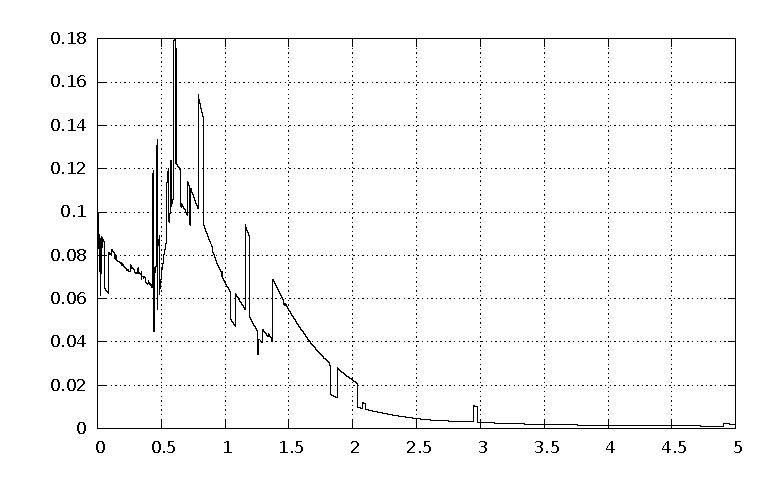
\includegraphics[width=.45\textwidth]
{figures/stokes/nonuniform_bubble_velocity_32_both.ps}
\caption[Stokes equidistribution velocity]
{($\mu=\gamma=1$) $\|\vec U^m\|_{L^\infty(\Omega)}$ evolution for a nonuniform
circle formed by $J_\Gamma = 32$ elements. Here we use the P2--P0 element, and
let $C_v = 3$.}
\label{fig:nonuniform_bubble_velocity_32_both}
\end{figure}

Finally, we would also like to investigate the effect of using an adaptive bulk
mesh, which is more refined close to the interface, and performing only mesh
smoothing. We use $J_\Gamma = 64$ elements for $\Gamma^0$ and $J_\Omega^0 =
954$ elements for the bulk. We see from the evolution in
Figure~\ref{fig:nonuniform_bubble_64_adaptive} that, again, we obtain an
equidistributed approximation of a circle. Obviously, since we never perform a
remesh, the final bulk mesh quality is very poor.
\begin{figure}[htbp]
\centering
\subfloat[$t=0$]{\includegraphics[width=.45\textwidth]
{figures/stokes/nonuniform_bubble_64_coarse_smooth_000.ps}}\\
\subfloat[$t=0.5$]{\includegraphics[width=.45\textwidth]
{figures/stokes/nonuniform_bubble_64_coarse_smooth_050.ps}}
\subfloat[$t=1$]{\includegraphics[width=.45\textwidth]
{figures/stokes/nonuniform_bubble_64_coarse_smooth_100.ps}}\\
\subfloat[$t=2.5$]{\includegraphics[width=.45\textwidth]
{figures/stokes/nonuniform_bubble_64_coarse_smooth_250.ps}}
\subfloat[$t=5$]{\includegraphics[width=.45\textwidth]
{figures/stokes/nonuniform_bubble_64_coarse_smooth_500.ps}}
\caption[Stokes equidistribution property adaptive mesh]
{($\mu=\gamma=1$) Mesh evolution of a nonuniform circle formed by
$J_\Gamma = 64$ elements and adaptive bulk mesh. Here we use the P2--P0
element, and no remeshing.}
\label{fig:nonuniform_bubble_64_adaptive}
\end{figure}
In Figure~\ref{fig:nonuniform_bubble_velocity_64_coarse_smooth} is shown the
evolution of $\|\vec U^m\|_{L^\infty(\Omega)}$ which, again, converges to zero.
\begin{figure}[htbp]
\centering
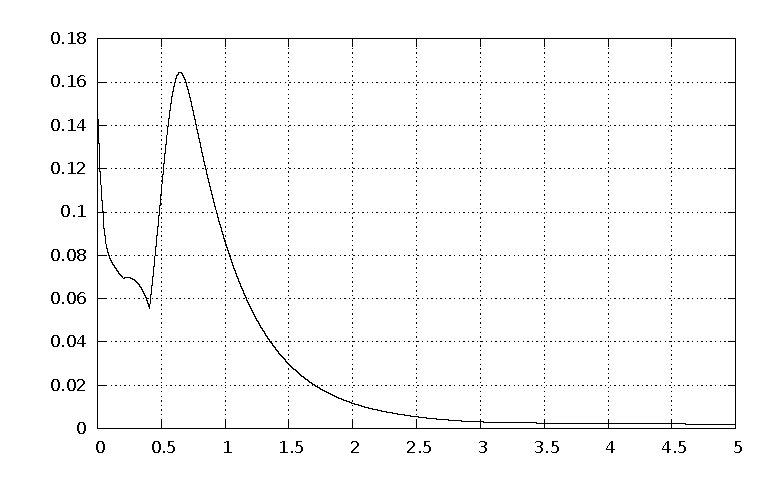
\includegraphics[width=.45\textwidth]
{figures/stokes/nonuniform_bubble_velocity_64_coarse_smooth.ps}
\caption[Stokes equidistribution velocity adaptive mesh]
{($\mu=\gamma=1$) $\|\vec U^m\|_{L^\infty(\Omega)}$ evolution for a nonuniform
circle formed by $J_\Gamma = 64$ elements and adaptive bulk mesh. Here we use
the P2--P0 element, and no remeshing.}
\label{fig:nonuniform_bubble_velocity_64_coarse_smooth}
\end{figure}
We notice that the evolution of the quantity $\|\vec U^m\|_{L^\infty(\Omega)}$
is now very smooth respect to the one reported in
Figure~\ref{fig:nonuniform_bubble_32_both} but this is not surprising since we
never perform a remesh.

\section{Energy decay and area conservation in 2d}\label{sec:stokes_2d_energy}
In Figure~\ref{fig:ellipse_both} we show the pressure evolution for a
simulation that starts with an initial ellipse, with major and minor axes of
1.6 and 0.75. We use the parameters $\mu = \gamma=1$, $\tau=10^{-2}$ and
$T=10$. The initial interface is discretized with $J_\Gamma = 40$ surface
elements while the initial bulk mesh is nearly uniform and it has $J_\Omega^0 =
1112$ elements. We employ the P2--P0 element and use the remeshing parameter
$C_v=3$ during the evolution. Figure~\ref{fig:ellipse_both_volumes} shows the
evolution of the relative inner area
$\frac{\mathcal{L}^2(\Omega^m_-)}{\mathcal{L}^2(\Omega^0_-)}$ and the
evolution of the interface energy $\gamma\,\mathcal{H}^{1}(\Gamma^m)$. The
graphs show that the inner area is nearly conserved, and that the interface
energy is monotonically decreasing. We point out that, since there is no exact
solution to the problem, we cannot show the pressure state at time $t=0$
therefore we show the pressure state at $t=10^{-5}$, which is computed with the
help of our scheme with one time step of size $\tau=10^{-5}$.
\begin{figure}[htbp]
\centering
\subfloat[$t=10^{-5}$]{\includegraphics[width=.45\textwidth]
{figures/stokes/ellipse_both_000.ps}}\\
\subfloat[$t=2.5$]{\includegraphics[width=.45\textwidth]
{figures/stokes/ellipse_both_250.ps}}
\subfloat[$t=5$]{\includegraphics[width=.45\textwidth]
{figures/stokes/ellipse_both_500.ps}}\\
\subfloat[$t=7.5$]{\includegraphics[width=.45\textwidth]
{figures/stokes/ellipse_both_750.ps}}
\subfloat[$t=10$]{\includegraphics[width=.45\textwidth]
{figures/stokes/ellipse_both_1000.ps}}
\caption[Stokes ellipse pressure]
{($\mu=\gamma=1$) Pressure evolution of an ellipse that evolves towards a
circle. Here we use the P2--P0 element, and let $C_v = 3$.}
\label{fig:ellipse_both}
\end{figure}
\begin{figure}[htbp]
\centering
\subfloat[$\frac{\mathcal{L}^2(\Omega^m_-)}{\mathcal{L}^2(\Omega^0_-)}$]{
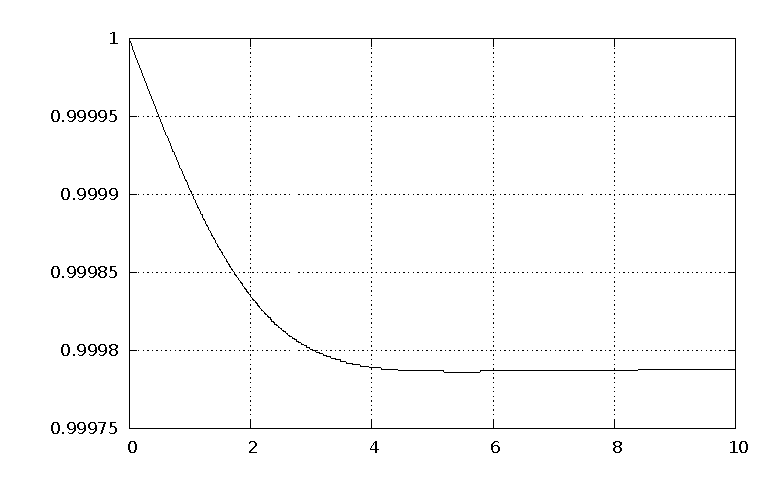
\includegraphics[width=.45\textwidth]
{figures/stokes/ellipse_both_bulk_inner_volume.ps}}
\subfloat[$\gamma\,\mathcal{H}^{1}(\Gamma^m)$]{
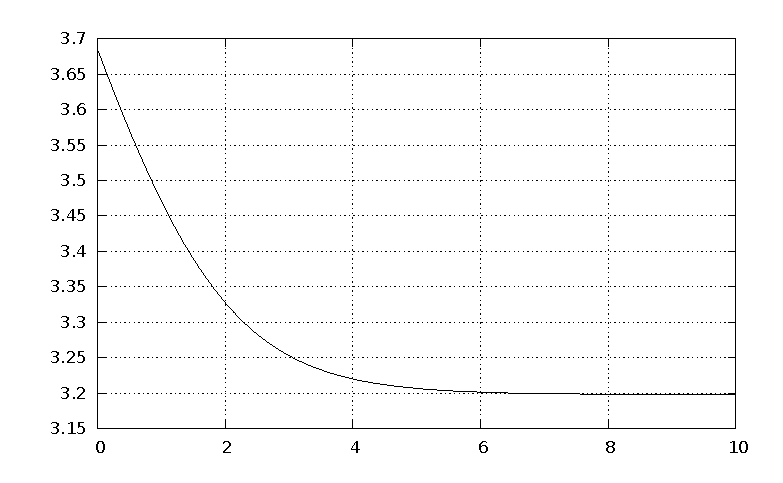
\includegraphics[width=.45\textwidth]
{figures/stokes/ellipse_both_interface_length.ps}}
\caption[Stokes ellipse inner area and interface energy]
{Evolutions of the relative inner area and the interface energy for
the simulation in Figure~\ref{fig:ellipse_both}.}
\label{fig:ellipse_both_volumes}
\end{figure}

As a comparison, we show in Figure~\ref{fig:ellipse_smooth} and
\ref{fig:ellipse_both_volumes_smooth} the same simulation when no remeshings are
performed, i.e. we use $C_v=\infty$ in (\ref{eq:volume_criterion}). We clearly
see that due to the strong deformation of the interface, this leads to
elongated elements in the inner and in the outer phase of the bulk finite
element mesh.
\begin{figure}[htbp]
\centering
\subfloat[$t=10^{-5}$]{\includegraphics[width=.45\textwidth]
{figures/stokes/ellipse_smooth_000.ps}}\\
\subfloat[$t=2.5$]{\includegraphics[width=.45\textwidth]
{figures/stokes/ellipse_smooth_250.ps}}
\subfloat[$t=5$]{\includegraphics[width=.45\textwidth]
{figures/stokes/ellipse_smooth_500.ps}}\\
\subfloat[$t=7.5$]{\includegraphics[width=.45\textwidth]
{figures/stokes/ellipse_smooth_750.ps}}
\subfloat[$t=10$]{\includegraphics[width=.45\textwidth]
{figures/stokes/ellipse_smooth_1000.ps}}
\caption[Stokes ellipse pressure no remeshing]
{($\mu=\gamma=1$) Pressure evolution of an ellipse that evolves towards a
circle. Here we use the P2--P0 element, and no remeshing.}
\label{fig:ellipse_smooth}
\end{figure}
\begin{figure}[htbp]
\centering
\subfloat[$\frac{\mathcal{L}^2(\Omega^m_-)}{\mathcal{L}^2(\Omega^0_-)}$]{
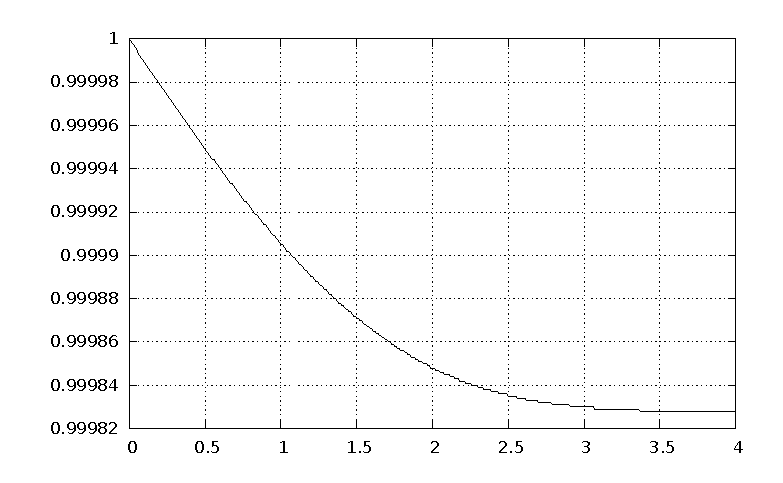
\includegraphics[width=.45\textwidth]
{figures/stokes/ellipse_smooth_bulk_inner_volume.ps}}
\subfloat[$\gamma\,\mathcal{H}^{1}(\Gamma^m)$]{
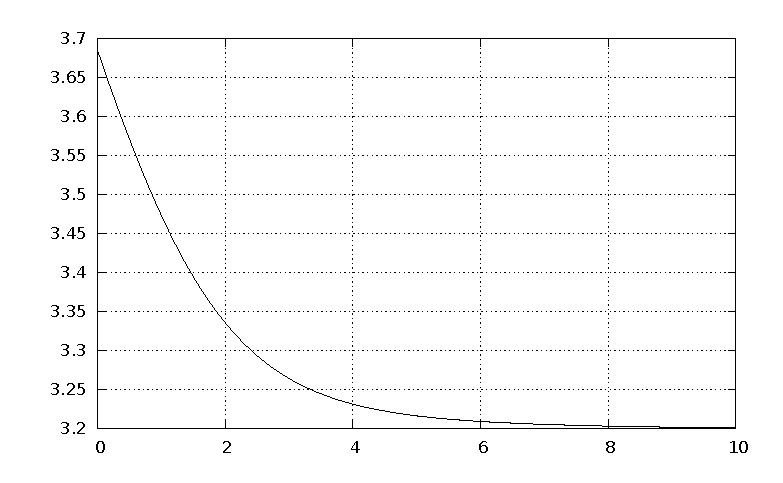
\includegraphics[width=.45\textwidth]
{figures/stokes/ellipse_smooth_interface_length.ps}}
\caption[Stokes ellipse inner area and interface energy no remeshing]
{Evolutions of the relative inner area and the interface energy for
the simulation in Figure~\ref{fig:ellipse_smooth}.}
\label{fig:ellipse_both_volumes_smooth}
\end{figure}

\section{Shear flow experiment in 2d}\label{sec:stokes_2d_shear}
As the final 2d numerical simulation we present a shear flow experiment. Here
we prescribe the inhomogeneous Dirichlet boundary condition
\begin{equation*}
\vec g(\vec z)=(z_2,0)^T\quad \mbox{on }\partial_1\Omega=\partial\Omega\,,
\end{equation*}
and we use the parameters $\mu=1$, $\gamma=3$, $\tau=10^{-2}$ and $T=5$.
The initial interface is discretized with $J_\Gamma = 64$ surface elements,
and the initial bulk mesh is nearly uniform with $J_\Omega^0 = 4240$ elements.
In Figure~\ref{fig:shear_2d} we show the evolution of the discrete pressures
for a simulation with $C_v=3$ for the P2--P0 element, while the velocities
are visualized in Figure~\ref{fig:shear_2d_velocity}.
\begin{figure}[htbp]
\centering
\subfloat[$t=0.5$]{\includegraphics[width=.45\textwidth]
{figures/stokes/2d_shear_050.ps}}
\subfloat[$t=1$]{\includegraphics[width=.45\textwidth]
{figures/stokes/2d_shear_100.ps}}\\
\subfloat[$t=2.5$]{\includegraphics[width=.45\textwidth]
{figures/stokes/2d_shear_250.ps}}
\subfloat[$t=5$]{\includegraphics[width=.45\textwidth]
{figures/stokes/2d_shear_500.ps}}
\caption[Stokes 2d shear flow pressure]
{($\mu=1,\gamma=3$) Pressure evolution for the 2d shear flow with $C_v=3$ for
the P2--P0 element, nearly uniform mesh.}
\label{fig:shear_2d}
\end{figure}
\begin{figure}[htbp]
\centering
\subfloat[$t=0.5$]{\includegraphics[width=.45\textwidth]
{figures/stokes/2d_shear_velocity_050.ps}}
\subfloat[$t=1$]{\includegraphics[width=.45\textwidth]
{figures/stokes/2d_shear_velocity_100.ps}}\\
\subfloat[$t=2.5$]{\includegraphics[width=.45\textwidth]
{figures/stokes/2d_shear_velocity_250.ps}}
\subfloat[$t=5$]{\includegraphics[width=.45\textwidth]
{figures/stokes/2d_shear_velocity_500.ps}}
\caption[Stokes 2d shear flow velocity]
{($\mu=1,\gamma=3$) Velocity vector field for the 2d shear flow with $C_v=3$
for the P2--P0 element, nearly uniform mesh.}
\label{fig:shear_2d_velocity}
\end{figure}

A plot of the relative inner area over time is shown in
Figure~\ref{fig:shear_2d_bulk_inner_volume}, where we again observe that our
numerical method maintains the enclosed volume well.
\begin{figure}[htbp]
\centering
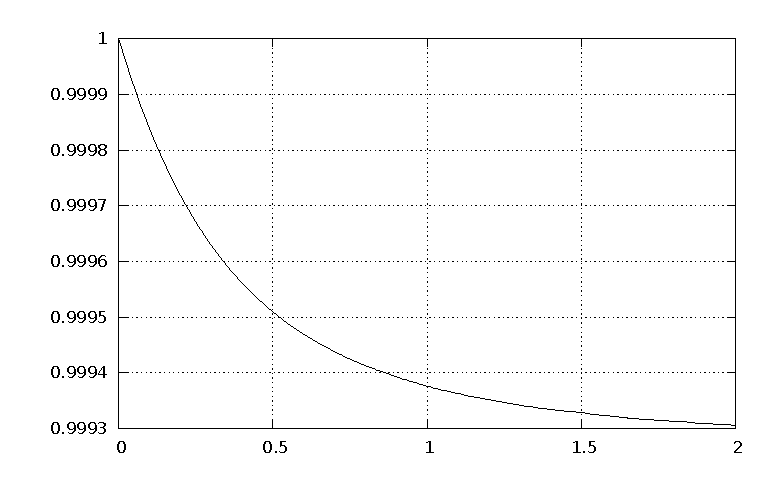
\includegraphics[width=.45\textwidth]
{figures/stokes/2d_shear_bulk_inner_volume.ps}
\caption[Stokes 2d shear flow inner area]
{A plot of the relative inner area
$\frac{\mathcal{L}^2(\Omega^m_-)}{\mathcal{L}^2(\Omega^0_-)}$
over time for the simulation in Figure~\ref{fig:shear_2d}.}
\label{fig:shear_2d_bulk_inner_volume}
\end{figure}

Finally we want to compare the performance of different preconditioner
for the preconditioned GMRES used to solve the reduce system
(\ref{eq:SchurkX}) or, depending on the pressure space,
(\ref{eq:SchurkX_extended}). In Table~\ref{tab:shear_2d_preconditioners} we
report the CPU time, in seconds, and the number of GMRES iteration to solve the
algebraic system (\ref{eq:SchurkX_extended}) at the first time step, $m=0$. We
employ nearly uniform bulk meshes and the P2--(P1+P0) element. We test the
direct preconditioner (\ref{eq:stokes_direct_precond_extended}) factorizing it
alternatively with either UMFPACK or SPQR and the block preconditioner
(\ref{eq:ESW_extended}) with restart value either 50 or 1000.
\begin{table*}
\center
\hspace*{-3.25cm}
\begin{tabular}{rrrrrrrrr}
\hline
$J_\Gamma$ & \multicolumn{2}{r}{Direct UMFPACK} &
\multicolumn{2}{r}{Direct SPQR} & \multicolumn{2}{r}{Block restart 50} &
\multicolumn{2}{r}{Block restart 1000} \\
\hline
 & CPU[s] & iterations & CPU[s] & iterations & CPU[s] & iterations & CPU[s] &
iterations \\
\hline
 16 &  0.06 & 6 &  0.13 & 5 &    0.94 &  349 &    1.16 &  221 \\
 32 &  0.33 & 7 &  0.68 & 6 &   11.33 &  839 &   11.51 &  441 \\
 64 &  1.83 & 8 &  4.16 & 8 &  138.58 & 2026 &  136.99 &  772 \\
128 & 10.05 & 9 & 25.71 & 9 & 2079.82 & 6436 & 1442.76 & 1745 \\
\hline
\end{tabular}
\hspace*{-3.25cm}
\caption[Stokes 2d shear flow preconditioners comparison]
{($\mu=1,\gamma=3$) Time and number of GMRES iterations to solve the algebraic
system (\ref{eq:SchurkX_extended}) adopting different preconditioners for the 2d
shear flow using P2--(P1+P0) element, nearly uniform mesh and $m=0$.}
\label{tab:shear_2d_preconditioners}
\end{table*}
We can notice that the direct preconditioner, whose matrix is equivalent to
the standard Stokes discretization (\ref{eq:stokes_system}) perform extremely
well in terms of CPU time and number of GMRES iterations. This is not very
surprising since the preconditioner and the reduced two-phase stokes system
have almost the same matrix. Therefore the number of GMRES iterations is very
low. Moreover, the factorization is computed only once with both SPQR and
UMFPACK so it is extremely efficient to apply the preconditioner at every GMRES
iteration. On the other hand, the block preconditioner perform very poorly
requiring a very high number of GMRES iterations in order to converge. An
increase of the restart value obviously reduce the number of GMRES iterations
but also drastically increase the memory footprint. Moreover, the application
of the preconditioner consist of doing the backward substitution
(\ref{eq:blocksolution_extended}) which is expensive.

\section{Convergence test in 3d}\label{sec:stokes_3d_convergence_results}
Similarly to \S\ref{sec:stokes_2d_convergence_results}, we perform the following
convergence test for a stationary spherical bubble in 3d. Let $\mu = \gamma =
1$. Then the true solution (\ref{eq:radialr},b) reduces to $r(t) =
\frac{1}{2}$, $\vec u(\cdot, t) = \vec 0$ and $p(t) = 4\,\charfcn{\Omega_-(0)}
- \frac{\pi}{12}$ for all $t\geq0$. We approximate this stationary solution on
nearly uniform meshes that feature $J_\Gamma = 32$, $220$ and $596$ interface
elements, and $J_\Omega^0 = 408$, $3590$ and $20473$ bulk elements,
respectively. Here, in contrast to the situation in 2d, we are not able to
define $\Gamma^0$ such that the vertices of $\Gamma^0$ lie on $\Gamma(0)$ and
such that (\ref{eq:constcurv}) is satisfied. As we would like to demonstrate
the ability of our method to recover the discrete stationary solution
(\ref{eq:solsol}) also in 3d, we choose the initial interface $\Gamma^0$ such
that (\ref{eq:constcurv}) holds, at the expense of a nonzero initial error
$\| \Gamma^0 - \Gamma(0) \|_{L^\infty}$, recall (\ref{eq:errorXx}). We obtain
such an initial triangulation with the help of the numerical scheme
(\ref{eq:fem_surf_diff_a}--b)from Chapter~\ref{ch:geometric_pdes} for surface
diffusion, which is a gradient flow for surface area that maintains the
enclosed volume. See Figure~\ref{fig:conformal_sphere}, or
\cite[Fig. 11]{gflows3d}, for an evolution towards a polyhedral approximation
of a sphere that satisfies (\ref{eq:constcurv}), and hence also
(\ref{eq:conformal}). The sphere in Figure~\ref{fig:conformal_sphere} has
$J_\Gamma = 596$ elements.
\begin{figure}[htbp]
\centering
\subfloat[Initial sphere triangulation]
{\includegraphics[width=.45\textwidth]{figures/stokes/sphere_596.ps}}
\subfloat[Conformal polyhedral sphere triangulation]
{\includegraphics[width=.45\textwidth]{figures/stokes/sphere_stationary_596.ps}}
\caption[Conformal polyhedral sphere triangulation]{Initial triangulation of
a sphere and conformal polyhedral sphere after surface diffusion.}
\label{fig:conformal_sphere}
\end{figure}

We report on the errors for the P2--P0, P2--P1, P2--\pdg and P2--(P1+P0)
elements in Tables~\ref{tab:stokes_stationary_3d_p2p0},
\ref{tab:stokes_stationary_3d_p2p1}, \ref{tab:stokes_stationary_3d_p2p1dg} and
\ref{tab:stokes_stationary_3d_p2p1p0}, respectively. Here we note that, as yet,
for the pairs P2--P0, P2--\pdg and P2--(P1+P0) there exist no proofs in the
literature that the LBB condition (\ref{eq:LBB}) holds, see e.g. the discussion
in \cite[Remark~8.4.3]{BoffiBF13}. However, in practice we encountered no
problems when using these spaces, and our iterative solver always converged to a
solution of the scheme (\ref{eq:HGa}--d). For both sets of simulations we use
the uniform time step size $\tau = 10^{-2}$.
\begin{table*}
\center
\begin{tabular}{rllllr}
\hline
$J_\Gamma$ & $\errorXx$ & $\LerrorUu2$ & $\LerrorPp$ & EOC & CPU[s] \\
\hline
 32 & 2.97986e-02 & 0 & 1.65555e-00 &    - &   385 \\
220 & 5.80971e-03 & 0 & 7.14269e-01 & 1.21 &  4699 \\
596 & 2.42857e-03 & 0 & 3.58466e-01 & 0.99 & 51604 \\
\hline
\end{tabular}
\caption[Stokes 3d stationary bubble errors P2--P0]
{($\mu=\gamma=1$) Stationary bubble problem on $(-1,1)^3$ over the time
interval $[0,1]$ for the P2--P0 element.}
\label{tab:stokes_stationary_3d_p2p0}
\end{table*}
\begin{table*}
\center
\begin{tabular}{rllllr}
\hline
$J_\Gamma$ & $\errorXx$ & $\LerrorUu2$ & $\LerrorPp$ & EOC & CPU[s] \\
\hline
 32 & 1.56938e-01 & 6.01956e-02 & 2.10996e-00 &    - &   315 \\
220 & 7.28946e-02 & 3.13992e-02 & 1.47595e-00 & 0.52 &  4231 \\
596 & 4.04291e-02 & 1.34276e-02 & 1.09674e-00 & 0.43 & 51287 \\
\hline
\end{tabular}
\caption[Stokes 3d stationary bubble errors P2--P1]
{($\mu=\gamma=1$) Stationary bubble problem on $(-1,1)^3$ over the time
interval $[0,1]$ for the P2--P1 element.}
\label{tab:stokes_stationary_3d_p2p1}
\end{table*}
\begin{table*}
\center
\begin{tabular}{rllllr}
\hline
$J_\Gamma$ & $\errorXx$ & $\LerrorUu2$ & $\LerrorPp$ & EOC & CPU[s] \\
\hline
 32 & 2.97986e-02 & 0 & 1.65555e-00 &    - &    73 \\
220 & 5.80971e-03 & 0 & 7.14269e-01 & 1.21 &  1018 \\
596 & 2.42857e-03 & 0 & 3.58466e-01 & 0.99 & 17814 \\
\hline
\end{tabular}
\caption[Stokes 3d stationary bubble errors P2--\pdg]
{($\mu=\gamma=1$) Stationary bubble problem on $(-1,1)^3$ over the time
interval $[0,1]$ for the P2--\pdg element.}
\label{tab:stokes_stationary_3d_p2p1dg}
\end{table*}
\begin{table*}
\center
\begin{tabular}{rllllr}
\hline
$J_\Gamma$ & $\errorXx$ & $\LerrorUu2$ & $\LerrorPp$ & EOC & CPU[s] \\
\hline
 32 & 2.97986e-02 & 0 & 1.65749e-00 &    - &    568 \\
220 & 5.80971e-03 & 0 & 7.15353e-01 & 1.21 &   9174 \\
596 & 2.42857e-03 & 0 & 3.59181e-01 & 0.99 & 121110 \\
\hline
\end{tabular}
\caption[Stokes 3d stationary bubble errors P2--(P1+P0)]
{($\mu=\gamma=1$) Stationary bubble problem on $(-1,1)^3$ over the time
interval $[0,1]$ for the P2--(P1+P0) element.}
\label{tab:stokes_stationary_3d_p2p1p0}
\end{table*}

We note that we again recover the discrete stationary solutions
(\ref{eq:solsol}) for the P2--P0, P2--\pdg and P2--(P1+P0) elements while,
as before, the P2--P1 element does not capture exactly the true solution
since this element does not satisfy the hypothesis that
$\charfcn{\Omega^m_-}\in\pspace^m$ of Theorem~\ref{thm:stat2}. Here this leads
to a nonzero error in the position of the discrete interface, because the
vertices of the initial interface $\Gamma^0$ do not lie on $\Gamma(0)$.

\section{Shear flow experiment in 3d}\label{sec:stokes_3d_shear}
Finally, we also report on a 3d shear flow experiment. The initial interface
mesh has $J_\Gamma = 596$ elements, while the nearly uniform bulk mesh is made
up of $J_\Omega^0 = 19641$ elements. We prescribe the inhomogeneous Dirichlet
boundary condition
\begin{equation*}
\vec g(\vec z)=(z_3,0,0)^T\quad \mbox{on }\partial_1\Omega=\partial\Omega\,,
\end{equation*}
and we use the parameters $\mu=1$, $\gamma=3$, $\tau=10^{-2}$ and $T=5$.
In Figure~\ref{fig:shear_3d} we show the evolution of the discrete interface
for a simulation with $C_v=3$ for the P2--P0 element, while the velocities
are visualized in Figure~\ref{fig:shear_3d_velocity}.
\begin{figure}[htbp]
\centering
\subfloat[$t=0$]{\includegraphics[width=.45\textwidth]
{figures/stokes/3d_shear_000.ps}}\\
\subfloat[$t=0.5$]{\includegraphics[width=.45\textwidth]
{figures/stokes/3d_shear_050.ps}}
\subfloat[$t=1$]{\includegraphics[width=.45\textwidth]
{figures/stokes/3d_shear_100.ps}}\\
\subfloat[$t=2.5$]{\includegraphics[width=.45\textwidth]
{figures/stokes/3d_shear_250.ps}}
\subfloat[$t=5$]{\includegraphics[width=.45\textwidth]
{figures/stokes/3d_shear_500.ps}}
\caption[Stokes 3d shear flow interface]
{($\mu=1,\gamma=3$) Interface evolution for the 3d shear flow with $C_v=3$ for
the P2--P0 element, nearly uniform mesh.}
\label{fig:shear_3d}
\end{figure}
\begin{figure}[htbp]
\centering
\subfloat[$t=0.5$]{\includegraphics[width=.45\textwidth]
{figures/stokes/3d_shear_velocity_050.ps}}
\subfloat[$t=1$]{\includegraphics[width=.45\textwidth]
{figures/stokes/3d_shear_velocity_100.ps}}\\
\subfloat[$t=2.5$]{\includegraphics[width=.45\textwidth]
{figures/stokes/3d_shear_velocity_250.ps}}
\subfloat[$t=5$]{\includegraphics[width=.45\textwidth]
{figures/stokes/3d_shear_velocity_500.ps}}
\caption[Stokes 3d shear flow velocity]
{($\mu=1,\gamma=3$) Velocity vector field in the plane normal to $(0,1,0)^T$
and passing through the origin for the 3d shear flow with $C_v=3$ for the
P2--P0 element, nearly uniform mesh.}
\label{fig:shear_3d_velocity}
\end{figure}

A plot of the relative inner volume over time is shown in
Figure~\ref{fig:shear_3d_bulk_inner_volume}, where we again observe that our
numerical method maintains the enclosed volume well.
\begin{figure}[htbp]
\centering
\includegraphics[width=.45\textwidth]
{figures/stokes/3d_shear_bulk_inner_volume.ps}
\caption[Stokes 3d shear flow inner volume]
{A plot of the relative inner volume
$\frac{\mathcal{L}^3(\Omega^m_-)}{\mathcal{L}^3(\Omega^0_-)}$
over time for the simulation in Figure~\ref{fig:shear_3d}.}
\label{fig:shear_3d_bulk_inner_volume}
\end{figure}

Finally, as in the 2d case, see Table~\ref{tab:shear_2d_preconditioners}, we
want to compare the performance of different preconditioners. In
Table~\ref{tab:shear_3d_preconditioners} we report the CPU time, in seconds,
and the number of GMRES iteration to solve the algebraic system
(\ref{eq:SchurkX_extended}) at the first time step, $m=0$. We employ adaptive
bulk meshes and the P2--(P1+P0) element. We test the direct preconditioner
(\ref{eq:stokes_direct_precond_extended}) factorizing it alternatively with
either UMFPACK or SPQR and the block preconditioner (\ref{eq:ESW_extended})
with restart value either 50 or 1000.
\begin{table*}
\center
\hspace*{-3.25cm}
\begin{tabular}{rrrrrrrrr}
\hline
$J_\Gamma$ & \multicolumn{2}{r}{Direct UMFPACK} &
\multicolumn{2}{r}{Direct SPQR} & \multicolumn{2}{r}{Block restart 50} &
\multicolumn{2}{r}{Block restart 1000} \\
\hline
 & CPU[s] & iterations & CPU[s] & iterations & CPU[s] & iterations & CPU[s] &
iterations \\
\hline
 32 &  0.16 & 8 &  0.26 & 5 &   1.10 & 158 &  1.17 & 130 \\
220 &  3.56 & 7 &  4.91 & 6 &  15.31 & 234 & 14.53 & 193 \\
596 & 13.77 & 6 & 44.44 & 6 & 101.53 & 328 & 93.00 & 266 \\
\hline
\end{tabular}
\hspace*{-3.25cm}
\caption[Stokes 3d shear flow preconditioners comparison]
{($\mu=1,\gamma=3$) Time and number of GMRES iterations to solve the algebraic
system (\ref{eq:SchurkX_extended}) adopting different preconditioners for the 3d
shear flow using P2--(P1+P0) element, adaptive mesh and $m=0$.}
\label{tab:shear_3d_preconditioners}
\end{table*}
We observe that also in 3d the direct preconditioners outperform the block
preconditioner both in term of GMRES iterations and CPU time.